\documentclass[tikz,border=2pt]{standalone}
\usepackage{amsmath}
\usepackage{pgfplots}
\pgfplotsset{compat=1.18}
\usetikzlibrary{arrows.meta}
\begin{document}
% Example 4.5 (adjacency): lines x1=4, -2x1+x2=6, -x1-x2=-3, x1-x2=1 meet in six corner points;
% feasible (4,3),(4,14),(-1,4),(2,1) (extreme points of V), infeasible (4,-1),(-7,-8).
% Corners on a common line are adjacent; the diagonal (4,3)-(-1,4) (distance sqrt(26)) is not, the edge (4,3)-(4,14) (length 11) is.
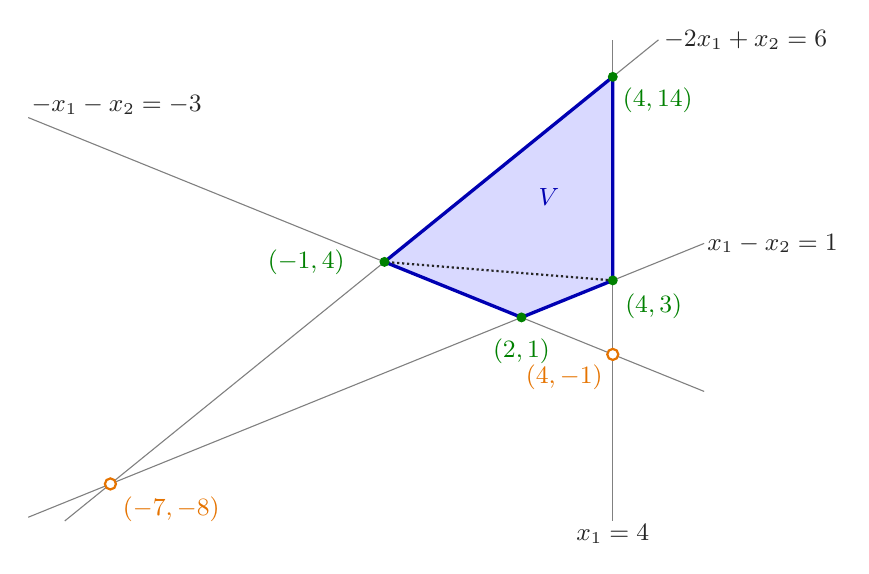
\begin{tikzpicture}[font=\small, >={Latex[length=2mm]}, x=0.58cm, y=0.235cm]
  \fill[blue!15] (2,1) -- (4,3) -- (4,14) -- (-1,4) -- cycle;
  % the four boundary lines
  \draw[gray] (4,-10) -- (4,16);
  \draw[gray] (-8,-10) -- (5,16);
  \draw[gray] (-8.8,11.8) -- (6,-3);
  \draw[gray] (-8.8,-9.8) -- (6,5);
  \node[gray!30!black, anchor=north, inner sep=1pt] at (4,-10) {$x_1=4$};
  \node[gray!30!black, anchor=west, inner sep=1pt] at (5.05,16) {$-2x_1+x_2=6$};
  \node[gray!30!black, anchor=south west, inner sep=1pt] at (-8.8,11.8) {$-x_1-x_2=-3$};
  \node[gray!30!black, anchor=west, inner sep=1pt] at (6,5) {$x_1-x_2=1$};
  % boundary of V: edges between adjacent feasible corners
  \draw[blue!70!black, very thick] (2,1) -- (4,3) -- (4,14) -- (-1,4) -- cycle;
  % a nonadjacent pair
  \draw[gray!30!black, thick, densely dotted] (4,3) -- (-1,4);
  % corner points
  \foreach \p in {(4,3),(4,14),(-1,4),(2,1)} \fill[green!50!black] \p circle (1.8pt);
  \foreach \p in {(4,-1),(-7,-8)} \draw[orange!90!black, thick, fill=white] \p circle (2pt);
  \node[green!50!black, anchor=north west, inner sep=1pt] at (4.15,13.6) {$(4,14)$};
  \node[green!50!black, anchor=west, inner sep=1pt] at (4.2,1.6) {$(4,3)$};
  \node[green!50!black, anchor=east, inner sep=1pt] at (-1.8,4) {$(-1,4)$};
  \node[green!50!black, anchor=north, inner sep=1pt] at (2,0) {$(2,1)$};
  \node[orange!90!black, anchor=north east, inner sep=1pt] at (3.85,-1.4) {$(4,-1)$};
  \node[orange!90!black, anchor=north west, inner sep=1pt] at (-6.8,-8.5) {$(-7,-8)$};
  \node[blue!70!black] at (2.6,7.5) {$V$};
\end{tikzpicture}
\end{document}
